\documentclass[tikz,border=2pt]{standalone}
\usepackage{amsmath}
\usetikzlibrary{arrows.meta}
\begin{document}
% Pooling two compound Poisson portfolios (rate 2, claims 10; rate 3, claims 20; illustrative arrival
% times): the pooled stream has rate 5 and a claim is 10 w.p. 2/5, 20 w.p. 3/5. Bar height = claim size.
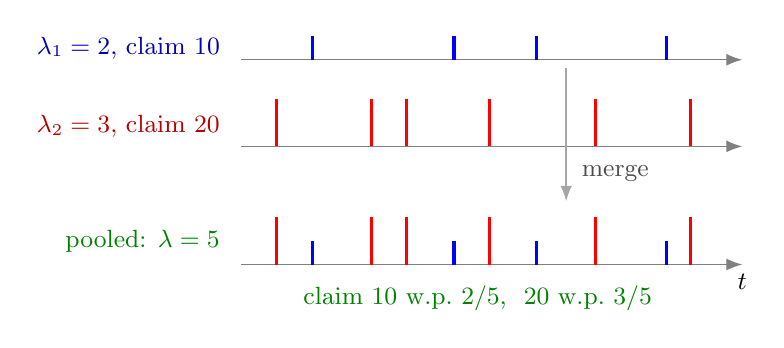
\begin{tikzpicture}[font=\small, >={Latex[length=2mm]}, x=3cm, y=1cm]
  \def\u{0.03}
  % portfolio 1
  \draw[->, gray] (0,2.6) -- (2.12,2.6);
  \foreach \t in {0.30,0.90,1.25,1.80} {\draw[blue, very thick] (\t,2.6) -- (\t,2.6+10*\u);}
  \node[blue!70!black, anchor=east] at (-0.05,2.75) {$\lambda_1=2$, claim $10$};
  % portfolio 2
  \draw[->, gray] (0,1.5) -- (2.12,1.5);
  \foreach \t in {0.15,0.55,0.70,1.05,1.50,1.90} {\draw[red, very thick] (\t,1.5) -- (\t,1.5+20*\u);}
  \node[red!70!black, anchor=east] at (-0.05,1.75) {$\lambda_2=3$, claim $20$};
  % pooled
  \draw[->, gray] (0,0) -- (2.12,0) node[below, black] {$t$};
  \foreach \t in {0.30,0.90,1.25,1.80} {\draw[blue, very thick] (\t,0) -- (\t,10*\u);}
  \foreach \t in {0.15,0.55,0.70,1.05,1.50,1.90} {\draw[red, very thick] (\t,0) -- (\t,20*\u);}
  \node[green!50!black, anchor=east, align=right] at (-0.05,0.3) {pooled: $\lambda=5$};
  \node[green!50!black, anchor=north] at (1.0,-0.15) {claim $10$ w.p.\ $2/5$,\ \ $20$ w.p.\ $3/5$};
  \draw[->, gray!70, thick] (1.375,2.5) -- (1.375,0.8);
  \node[gray!60!black, anchor=west] at (1.4,1.15) {merge};
\end{tikzpicture}
\end{document}
